\section{Numerical experiments}\label{sec:numerics}
Having constructed SSP $TM^{n-2}R$ schemes in the previous
section, we now numerically verify their properties.
%where $M$ is an ESSPRK($s,q,p$) scheme and
%$R$ and $T$ are its associated SSP starting and stopping schemes from
%Section~\ref{subsec:starting_stopping}.
Specifically, we use a convergence study to show that the procedure
attains order $q$.  We also demonstrate on Burgers' equation that the
SSP coefficient accurately measures the maximal stepsize for which the
methods are strong stability preserving.
%
% For simplicity we denote the multi-method $TM^{n-2}R$ procedure as an
% \emph{ESSPRK-scheme}.
\colintodo{I removed the new notation that was here: it was only used three times}

\subsection{Convergence study}\label{subsec:convergence}
We consider the nonlinear ODE
\begin{align}\label{eq:conv_eq}
    u'(t) = -\frac{3}{2}u^{2}(t), \quad t \in [0,1], \quad \text{with } u(0) = 10,
\end{align}
and exact solution $u(t) = 10/(15t + 1)$.
We solve the initial value problem \eqref{eq:conv_eq}
using SSP $TM^{n-2}R$ schemes.
% where $M$ is effective order three and four and classical order two.
The solution is computed for using $n = 50 \cdot 2^{k}$ time steps for
$k = 0, 1, 2, \dots, 6$.
% and 
%hence the time-step used is $\Dt = \tfrac{1}{N} = \tfrac{2^{(1-k)}}{100}$ 
%for each computation. 
The error at $t=1$ between the exact solution and the approximation with 
respect to time-step is shown in Figure~\ref{fig:conv_study} on a logarithmic 
scale.
\begin{figure}
	\centering
     \subfloat[SSPRK($s,3,2$)]{\label{fig:conv_study_a}
     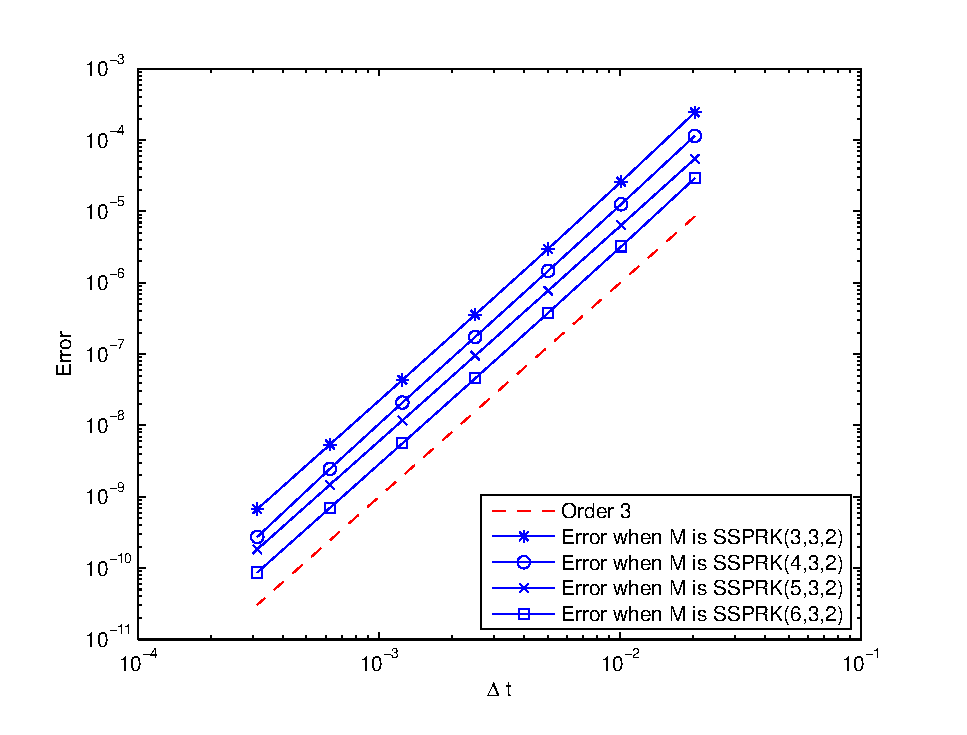
\includegraphics[width=0.45\textwidth]{Pictures/convergence_3rd_ord}}
   \quad
     \subfloat[SSPRK($s,4,2$)]{\label{fig:conv_study_b}
    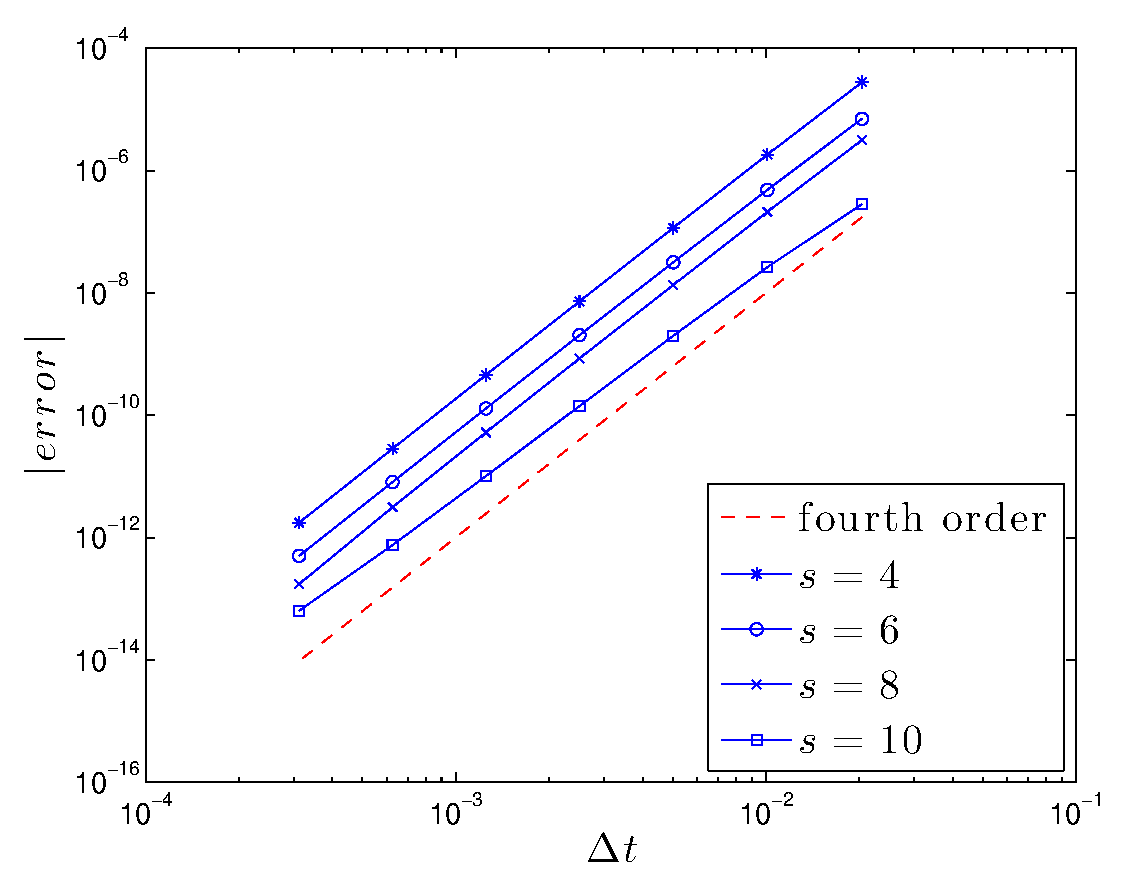
\includegraphics[width=0.45\textwidth]{Pictures/convergence_4th_ord}}
    \caption{Convergence study of $TM^{n-2}R$ Runge--Kutta schemes when (a) $M$
    is an SSPRK($s,3,2$) method and (b) $ M $ is an SSPRK($s,4,2$) method.}
    \label{fig:conv_study}
\end{figure}
The convergence study was performed for $TM^{n-2}R$ schemes with
various number of stages $s$ and the results show that the schemes
attain an order of accuracy equal to the effective order of their main
method $M$.
It is important in doing this sort of convergence study that the
effective order can only be obtained after the stopping method is
applied.
Intermediate steps will typically only be order $p$ accurate (the classical
order of the main method).
Finally, we note that for a fixed time-step increasing the number of stages
generally decreases the error constant.

\subsection{Burgers' equation}\label{subsubsec:burgers}
The inviscid Burgers' equation consists of the hyperbolic conservation law
\begin{align}\label{eq:HCL}
    U_{t} + f(U)_{x} = 0,
\end{align}
with flux function $f(U) = \frac{1}{2}U^{2}$. 
We consider initial data
$U(0,x)  = \frac{1}{2} - \frac{1}{4}\sin{\pi x}$,
on a periodic domain $x \in [0,2)$.
The solution advances to the right where it eventually exhibits a shock. 
We perform a semi-discretization
using an upwind approximation to obtain the system of ODEs
\begin{align*}\label{eq:burgers_flux}
	\frac{\textrm{d}}{\textrm{d} t} u_i = \frac{f(u_{i}) - f(u_{i-1})}{\Delta x}.
\end{align*}
This spatial discretization is total-variation-diminishing (TVD) when
coupled with Forward Euler method under time restriction
$\Dt \leq {\Dt}_{\text{FE}} = (1 / \|U(0,x)\|_{\infty}) \Delta x$
\cite{Laney:1998} %,Ketcheson/Macdonald/Gottlieb:2009}.
\colintodo{David: who would you cite: \textbf{Spatial disc being TVD}?}
Recall that a time discretization with SSP
coefficient $\sspcoef$, will give a TVD solution for $\Dt \leq
\sspcoef {\Dt}_{\text{FE}}$.

\colintodo{Is there a particular reason we use ESSPRK($10,4,2$)?  $(4,4,2)$ would seem more interesting/reproducible.}
\yiannistodo{No, I can change that.}
Burgers' equation was solved using an SSP $TM^{n-2}R$ scheme with time-step
restriction $\Dt \leq \sigma{\Dt}_{\text{FE}}$, where $\sigma$ indicates the size 
of the time step. 
We integrate to roughly time $t_{f} = 2.5$
with $m = 256$ points in space.
Figure~\ref{fig:burgers_cont} shows that if $\sigma$ stays below the SSP 
coefficient of the main method, then no oscillations are observed. 
If this stability limit is violated, then oscillations may appear.
\begin{figure}
    \centering
    \subfloat[$\sigma = 6.0$]{\label{fig:burgers_cont_a}
      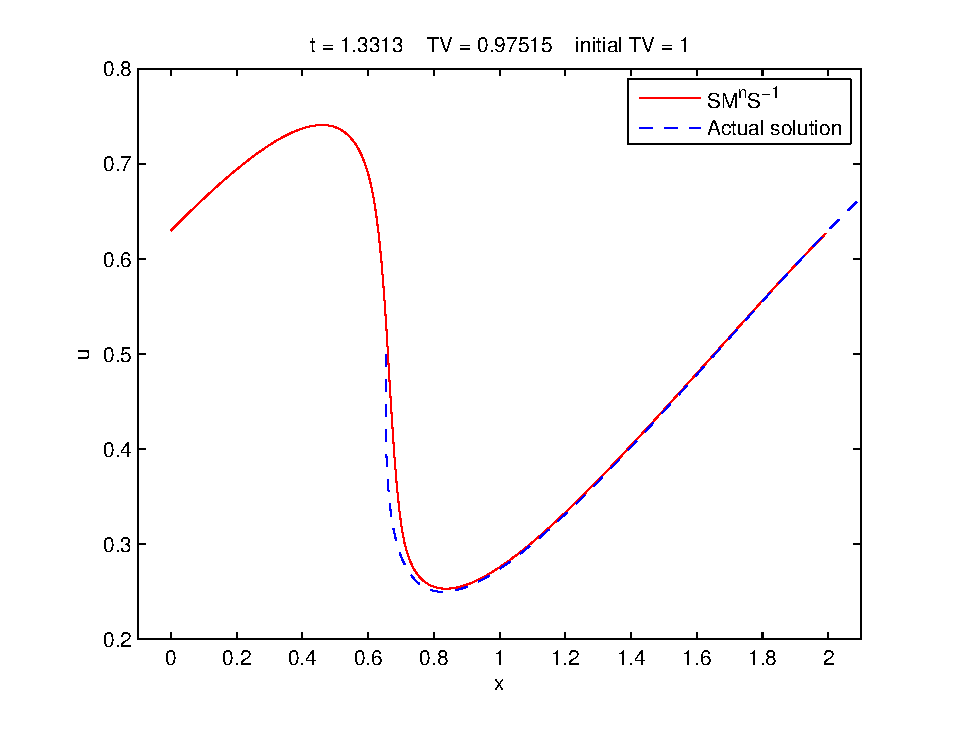
\includegraphics[width=0.45\textwidth]{Pictures/burgers_cont_tvd}}
    \quad
    \subfloat[$\sigma = 6.68$]{\label{fig:burgers_cont_b}
      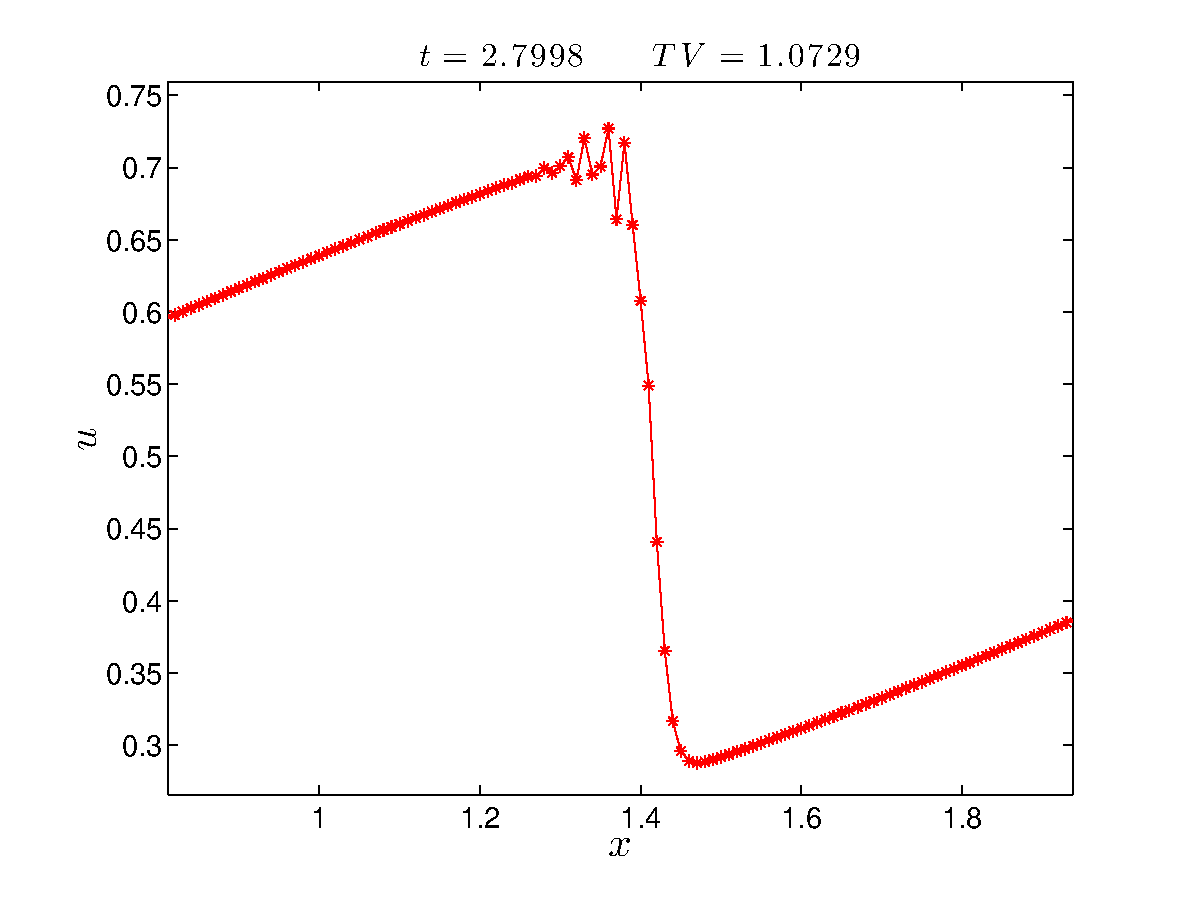
\includegraphics[width=0.45\textwidth]{Pictures/burgers_cont_no_tvd}}
    \caption{Solution of Burgers' equation with continuous initial data, using a 
    $TM^{n-2}R$ scheme, where $ M $ is ESSPRK($10,4,2$). 
    The SSP coefficient is $\sspcoef = 6.0$. 
    Here $TV$ denotes the difference between the $TV$-norms of the final and 
    initial solution.
    A positive sign indicates a violation of the TVD condition.}
    \label{fig:burgers_cont}
\end{figure}
%\yiannistodo{Elaborate more: Sharpness of SSP coefficient} 
%We were able to determine when exactly the nonlinear stability is not 
%satisfied by computing the the total-variation (TV) norm at each step of the 
%computation process. 
%This indicates that the ESSPRK-scheme inherits the time-step restriction 
%from the SSP coefficient of the main method $M$.
We measure these oscillations by computing the total variation of the 
numerical solution.
It turns out that \textbf{\red TODO $\sigma = x.yz$}
is the largest value of $\sigma$ for which the total variation has not
increased at the final time.
This is \textbf{\red TODO $xy\%$} larger the value SSP coefficient
$\sspcoef = 6$.
\colintodo{In the figures, I would prefer to just report the TV
  itself, instead of this TV error.}
 \yiannistodo{Fine, I fix this.}

We also consider Burgers' equation with a discontinuous
square wave initial condition
\begin{align*}%\label{eq:burgers_discont_IC}
    U(0,x)  = \left\{
                \begin{array}{ll}
                  1, & \hbox{$0.5 \leq x \leq 1.5$} \\
                  0, & \hbox{otherwise.}
                \end{array}
              \right.
\end{align*}
Figure~\ref{fig:burgers_discont} shows the result of solving the 
discontinuous problem using an ESSPRK-scheme, where $M$ is an 
SSPRK($10,4,2$) method.
\begin{figure}
    \centering
    \subfloat[$\sigma = 6.0$]{\label{fig:burgers_discont_a}
      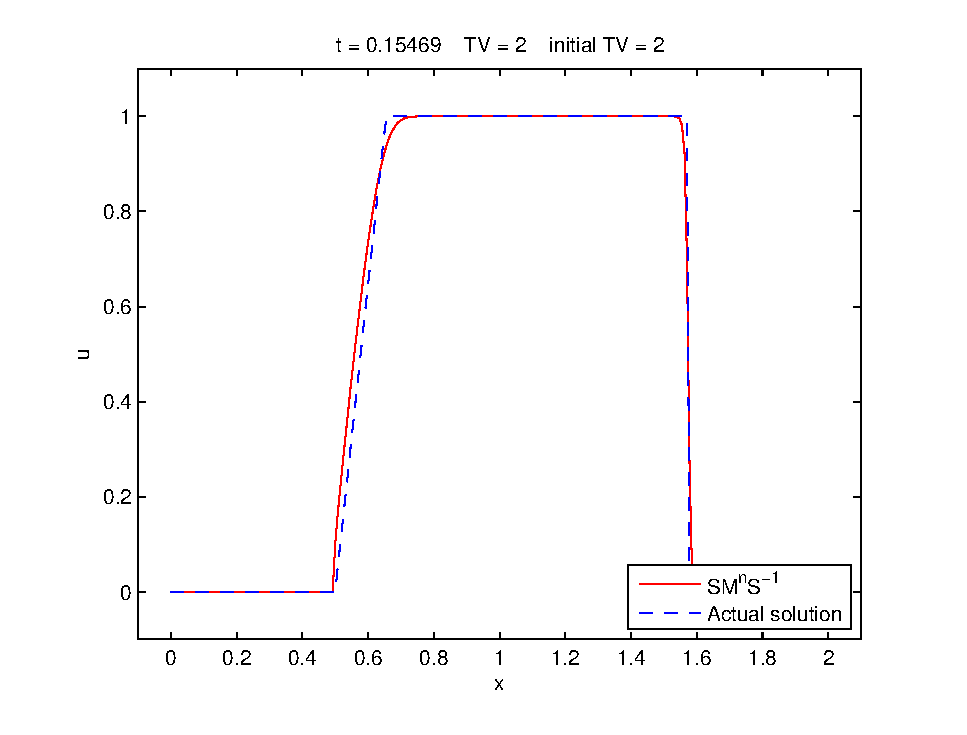
\includegraphics[width=0.45\textwidth]{Pictures/burgers_discont_tvd.eps}}
    \quad
    \subfloat[$\sigma = 6.18$]{\label{fig:burgers_discont_b}
      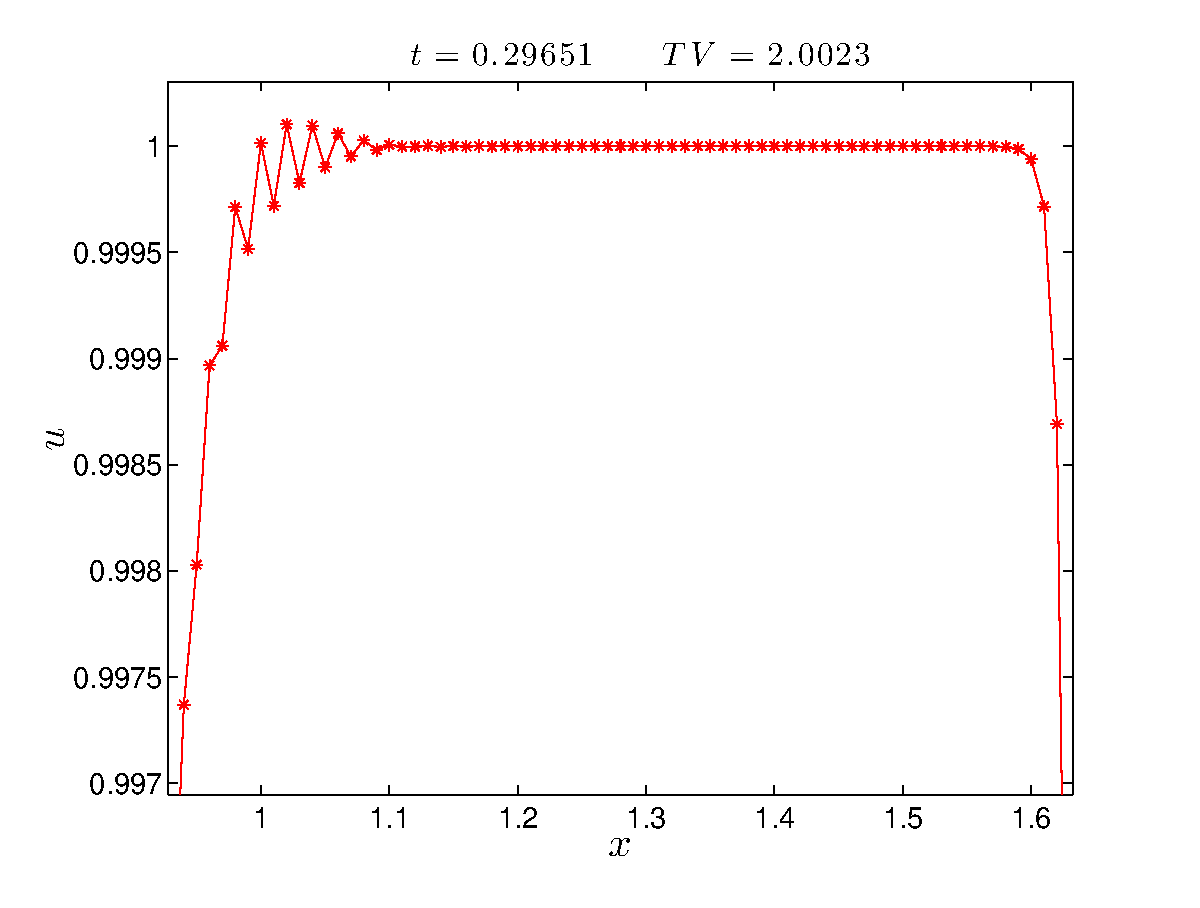
\includegraphics[width=0.45\textwidth]{Pictures/burgers_discont_no_tvd.eps}}
    \caption{Solution of Burgers' equation with discontinuous initial data, using a 
    $TM^{n-2}R$ scheme, where $M$ is SSPRK($10,4,2$) method. 
    The SSP coefficient is $ \sspcoef = 6.0$.
    Here $TV$ denotes the difference between the $TV$-norms of the final and 
    initial solution.
    A positive sign indicates a violation of the TVD condition.}
    \label{fig:burgers_discont}
\end{figure}
In this case, \textbf{\red TODO $\sigma = x.yz$} appears to be the
largest value of $\sigma$ for which the total variation has not
increased at the final time.
This is \textbf{\red TODO $xy\%$} larger than the SSP coefficient
$\sspcoef = 6$.

It is interesting to note that the stability prediction of the SSP
coefficient for ESSPRK is quite tight compared to other SSP methods
(c.f., \cite[Table 5.1]{Ketcheson/Gottlieb/Macdonald:TSRK}).
Also it becomes sharper as the number of spatial points increases,
since the dissipation of the solution is decreased. 
This may make effective order methods an interesting test case for
further research into both SSP time-discretizations as well as spatial
discretizations with strong stability features.

We also note the necessity of our $RM^{n-2}T$ approach: in this
example if we were to use the original approach of $S$ and $S^{-1}$,
the solution exhibits oscillations immediately following the
application of the starting perturbation scheme $S$.
%This is illustrated in Figure~\ref{fig:burgers_starting_method}
%\yiannistodo{Shall we include a plot about this?}
%Colin: fine as is for now

% The ESSPRK-scheme preserves monotonicity in the TV-norm since the starting 
% method $R$ is SSP.
% Using the original approach with $S$ and $S^{-1}$, the results are not
% SSP and the total-variation increases after the perturbation $S$.
% This is illustrated in Figure~\ref{fig:burgers_starting_method} in which 
% the solution is plotted after one application of methods $R$ and $S$ as the 
% starting procedures.
% % Note: its not really a step for %S% so I said application
% \begin{figure}
%     \centering
% 	TODO
% 	\yianniscomment{This should be cut out since if we optimize directly for R and T, we are not mentioning S.}
%     \caption{Solution of Burgers' equation with discontinuous initial data 
%     after one step, using a $TM^{n-2}R$ scheme, where $M$ is an 
%     SSPRK($5,4,2$) method. The solution is advanced one step by using (a) $R$ and 
%     (b) $S$}
%     \label{fig:burgers_starting_method}
% \end{figure}

